\documentclass{tufte-handout}

%\geometry{showframe}% for debugging purposes -- displays the margins



\newcommand{\bra}[1]{\left(#1\right)}

\usepackage{clrscode3e}
\usepackage[activate={true,nocompatibility},final,tracking=true,kerning=true,spacing=true,factor=1100,stretch=10,shrink=10]{microtype}
\usepackage{tikz}
\usetikzlibrary{calc,positioning}
\usepackage{amsmath,amsthm, amssymb}
\usepackage{enumitem}
\newenvironment{rcases}
{\left.\begin{aligned}}
{\end{aligned}\right\rbrace}
\usepackage{mathrsfs}
\usepackage[boxed,linesnumbered]{algorithm2e}
\usetikzlibrary{shapes}
\usetikzlibrary{positioning}
% Set up the images/graphics package
\usepackage{graphicx}
\setkeys{Gin}{width=\linewidth,totalheight=\textheight,keepaspectratio}
\graphicspath{{.}}

\title{Lecture Notes for CS 726 - Spring 2021}
\author[Eeshaan Jain]{Eeshaan Jain}
\date{\today}  % if the \date{} command is left out, the current date will be used

% The following package makes prettier tables.  We're all about the bling!
\usepackage{booktabs}
\usepackage{tikzit}
\input{sample.tikzstyles}
% The units package provides nice, non-stacked fractions and better spacing
% for units.
\usepackage{units}

% The fancyvrb package lets us customize the formatting of verbatim
% environments.  We use a slightly smaller font.
\usepackage{fancyvrb}
\fvset{fontsize=\normalsize}
% Small sections of multiple columns
\usepackage{multicol}
\usepackage{cancel}
\usepackage{xcolor}
\definecolor{DarkRed}{RGB}{139,0,0}
\usepackage{hyperref}
\hypersetup{colorlinks=true, linkbordercolor=DarkRed,linkcolor=DarkRed}
%--------Theorem Environments--------
%theoremstyle{plain} --- default
\newtheorem{thm}{Theorem}
\newtheorem{cor}[thm]{Corollary}
\newtheorem{prop}[thm]{Proposition}
\newtheorem{lem}[thm]{Lemma}
\newtheorem{conj}[thm]{Conjecture}
\newtheorem{quest}[thm]{Question}
\newtheorem{claim}{Claim}

\theoremstyle{definition}
\newtheorem{defn}[thm]{Definition}
\newtheorem{defns}[thm]{Definitions}
\newtheorem{con}[thm]{Construction}
\newtheorem{exmp}[thm]{Example}
\newtheorem{jk}[thm]{Joke}
\newtheorem{exmps}[thm]{Examples}
\newtheorem{notn}[thm]{Notation}
\newtheorem{notns}[thm]{Notations}
\newtheorem{addm}[thm]{Addendum}
\newtheorem{exer}[thm]{Exercise}

\theoremstyle{remark}
\newtheorem{rem}[thm]{Remark}
\newtheorem{ans}[thm]{Answer}
\newtheorem{rems}[thm]{Remarks}
\newtheorem{warn}[thm]{Warning}
\newtheorem{sch}[thm]{Scholium}

\newcommand{\ind}{\rotatebox[origin=c]{90}{$\models$}}
\newcommand{\Mod}[1]{\ (\text{mod}\ #1)}
\newcommand{\R}{\mathbb{R}}
\newcommand{\N}{\mathbb{N}}
\newcommand{\Q}{\mathbb{Q}}
\newcommand{\F}{\mathbb{F}}
\newcommand{\Z}{\mathbb{Z}}
\newcommand{\Prob}{\text{Pr}}
\renewcommand{\P}{\mathbb{P}}
\DeclareMathOperator{\Span}{Span}
\DeclareMathOperator{\val}{val}
\DeclareMathOperator{\comp}{comp}
\DeclareMathOperator{\im}{Im}
\DeclareMathOperator{\reg}{Reg}
\DeclareMathOperator{\odd}{Odd}
\DeclareMathOperator{\dist}{dist}
\DeclareMathOperator{\sbd}{sbd}
\DeclareMathOperator{\capac}{cap}


% These commands are used to pretty-print LaTeX commands
\newcommand{\doccmd}[1]{\texttt{\textbackslash#1}}% command name -- adds backslash automatically
\newcommand{\docopt}[1]{\ensuremath{\langle}\textrm{\textit{#1}}\ensuremath{\rangle}}% optional command argument
\newcommand{\docarg}[1]{\textrm{\textit{#1}}}% (required) command argument
\newenvironment{docspec}{\begin{quote}\noindent}{\end{quote}}% command specification environment
\newcommand{\docenv}[1]{\textsf{#1}}% environment name
\newcommand{\docpkg}[1]{\texttt{#1}}% package name
\newcommand{\doccls}[1]{\texttt{#1}}% document class name
\newcommand{\docclsopt}[1]{\texttt{#1}}% document class option name

\begin{document}
	
	\maketitle
	\begin{abstract}
		These are my lecture notes taken during the Advanced Machine Learning (CS 726) course at IIT Bombay during the Spring 2021 session.	\end{abstract}
	\tableofcontents
	\newpage
	\section{Probabilistic Modeling}
\subsection{Probability Theory}
\marginnote{In a single coin toss, we have \[\Omega = \{\text{H}, \text{T}\}\]}
We will briefly review probability in a rigorous sense. \\We define events considering we have a space of possible outcomes denoted by $\Omega$. $\mathcal S$ is a set of measurable events, to which we assign probabilities, and each event $\alpha \in \mathcal S$ is a subset of $\Omega$. \\
The event space necessarily satisfies three properties - 
\begin{enumerate}
	\item It contains the empty event $\emptyset$ and the trivial event $\Omega$.
	\item It is closed under union, i.e if $\alpha, \beta \in \mathcal S$, so is $\alpha \cup \beta$.
	\item It is closed under complementation, i.e if $\alpha \in \mathcal S$, so is $\Omega - \alpha$. 
\end{enumerate}
\begin{defn}[Probability distribution]\label{defn:prob}
A probability distribution $P$ over $(\Omega, \mathcal S)$ is a mapping of events in $\mathcal S$ to real values satisfying 
\marginnote{A direct consequence of the properties is: \[P(\emptyset) = 0\]\[P(\alpha \cup \beta) = P(\alpha) + P(\beta) - P(\alpha \cap \beta)\]}
\begin{itemize}[leftmargin=1cm]
	\item[$\diamond$] $P(\alpha) \geq 0$ for all $\alpha \in \mathcal S$
	\item[$\diamond$] $P(\Omega) = 1$
	\item[$\diamond$] If $\alpha, \beta \in \mathcal S$ and $\alpha \cap \beta = \emptyset$, then $P(\alpha \cup \beta) = P(\alpha) + P(\beta)$
\end{itemize}
\end{defn}
Conditional probability answers the question - after learning that event $\alpha$ is true, how does our belief about $\beta$ change? Formally, we define
\begin{equation}
	P(\beta|\alpha) = \dfrac{P(\alpha \cap \beta)}{P(\alpha)}
\end{equation}
It can be checked that this satisfies Definition \ref{defn:prob} and is a probability distribution. Noting that $P(\alpha \cap \beta) = P(\alpha) P(\beta|\alpha)$, we define the chain rule of conditional probabilities
\begin{equation}
P(\alpha_1 \cap \cdots\cap \alpha_k) = P(\alpha_1) P(\alpha_2|\alpha_1) \cdots P(\alpha_k|\alpha_1\cap\cdots\cap\alpha_{k-1})
\end{equation}
We further define the Bayes' rule
\begin{equation}\label{eqn:bayes}
P(\alpha|\beta) = \dfrac{P(\beta|\alpha)P(\alpha)}{P(\beta)}
\end{equation}
Here, $P(\alpha|\beta)$ is called the \textit{posterior}, $P(\beta|\alpha)$ is the \textit{likelihood}, $P(\alpha)$ is the \textit{prior} and $P(\beta)$ is the \textit{marginal probability} of the structure in context. We can generalize Equation \ref{eqn:bayes} as
\begin{equation}
P(\alpha|\beta \cap \gamma) = \dfrac{P(\beta|\alpha \cap \gamma)P(\alpha|\gamma)}{P(\beta|\gamma)}
\end{equation}
Now, we formally define the notion of random variables, which intuitively can be considered to be attribute reporters.
\begin{defn}[Random Variable]
	A random variable $X$ is a \textit{measurable} function $X:\Omega \to \mathcal S$. The probability that $X$ takes values in a set $s \in \mathcal S$ is written as
	\begin{equation}
		\text{Pr}(X \in s) = \text{Pr}(\{\omega \in \Omega|X(\omega) \in s\})
	\end{equation}
\end{defn}
The marginal distribution over a random variable $X$ is the distribution over events that can be described using $X$, and is denoted by $P(X)$. More generally, if we want to describe a distribution over a set of random variables $\mathcal X = \{x_1, \cdots, x_n\}$ called the \textit{joint distribution} denoted as $P(x_1, \cdots, x_n)$. The full assignment to the variables is denoted as $\xi \in \text{Val}(\mathcal X)$. The space corresponding to the joint assignment in $\mathcal X$ is called the \textit{canonical outcome space}. \\
Now, we glance at independencies, a core component of Probabilistic Graphical Models.
\begin{defn}[Independence]
An event $\alpha$ is independent of an event $\beta$ denoted by $P \models (\alpha\ind\beta)$, if $P(\alpha|\beta) = P(\alpha)$ or $P(\beta) = 0$.
\end{defn}
\begin{prop}
A distribution satisfies $(\alpha \ind \beta)$ if and only if 
\begin{equation}
P(\alpha\cap\beta) = P(\alpha)P(\beta)
\end{equation}
\end{prop}
\begin{proof}
Skipped (hint: Use the definition of conditional probability).
\end{proof}
\begin{defn}[Conditional Indpendence]
An event $\alpha$ is conditionally independent of event $\beta$ given $\gamma$ in $P$, denoted by $P \models (\alpha \ind\beta|\gamma)$ if $P(\alpha|\beta\cap\gamma) = P(\alpha|\gamma)$ or if $P(\beta\cap\gamma) = 0$.
\end{defn}
\begin{prop}
$P$ satisfies $(\alpha\ind\beta|\gamma)$ if and only if 
\begin{equation}
P(\alpha \cap\beta|\gamma) = P(\alpha|\gamma)P(\beta|\gamma)
\end{equation}
\end{prop}
\begin{defn}
Let $\mathbf{X, Y, Z}$ be sets of random variables. $\mathbf X$ is conditionally independent of $\mathbf Y$ given $\mathbf Z$ in a distribution $P$ if $P$ satisfies $(\mathbf X = \mathbf x \ind \mathbf Y = \mathbf y | \mathbf Z = \mathbf z)$ for all values of $\mathbf x \in \text{Val}(\mathbf X), \mathbf y \in \text{Val}(\mathbf Y)$ and $\mathbf z \in \text{Val}(\mathbf Z)$. We say that the variables in $\mathbf Z$ are \textit{observed}. If $\mathbf Z$ is empty, then we say that $\mathbf X$ and $\mathbf Y$ are marginally independent.
\end{defn}
\begin{prop}
The distribution $P$ satisfies $(\mathbf X \ind \mathbf Y|\mathbf Z)$ if and only if 
\begin{equation}
	P(\mathbf X,\mathbf Y|\mathbf Z) = P(\mathbf X|\mathbf Z)P(\mathbf Y|\mathbf Z)
\end{equation}
\end{prop}
The following properties hold for conditional independencies:
\begin{enumerate}
	\item \textit{Symmetry:} $(\mathbf X \ind \mathbf Y|\mathbf Z) \implies (\mathbf Y \ind \mathbf X|\mathbf Z)$
	\marginnote{Decomposition can also be stated as \[\mathbf{X\ind \{Y, Z\} \implies X\ind Y, X\ind Z}\]}
	\item \textit{Decomposition:} $(\mathbf X \ind \mathbf{Y, W}|\mathbf Z) \implies (\mathbf X \ind \mathbf Y|\mathbf{Z})$
	\marginnote{Weak Union can also be stated as \[\mathbf{X\ind \{Y, Z\} \implies X\ind Y|Z}\] But note that, if $\mathbf{X\ind Y}$ and $\mathbf{Z}\;\cancel\ind\;\{\mathbf{X,Y}\}$ then it is not necessary to have $\mathbf{X\ind Y|Z}$}
	\item \textit{Weak Union:} $(\mathbf X \ind \mathbf Y, \mathbf W|\mathbf Z) \implies (\mathbf X \ind \mathbf Y|\mathbf Z,  \mathbf W)$
	\item \textit{Contraction:} $(\mathbf X \ind \mathbf W|\mathbf Z, \mathbf Y)\; \& \;(\mathbf X \ind \mathbf Y|\mathbf Z) \implies (\mathbf X \ind \mathbf Y, \mathbf W|\mathbf Z)$
	\marginnote{Contraction can also be stated as \[\mathbf{X\ind Y|Z, X\ind Z \implies X\ind \{Y,Z\}}\]}
\end{enumerate}
If our distribution is positive (i.e, for all non-empty $\alpha \in \mathcal S, P(\alpha) > 0$), we have another property
\begin{itemize}[leftmargin=1cm]
	\item[$\diamond$] \textit{Intersection:}  $(\mathbf X \ind \mathbf Y|\mathbf Z, \mathbf W)\; \& \;(\mathbf X \ind \mathbf W|\mathbf Z, \mathbf Y) \implies (\mathbf X \ind \mathbf Y, \mathbf W|\mathbf Z)$
\end{itemize}
\begin{thm}\label{thm:factor}
Consider $\mathcal{X} = \mathbf{\{X, Y, Z\}}$. Then $P\models (\mathbf X \ind \mathbf Y | \mathbf Z)$ if and only if we can write 
\begin{equation}
P(\mathcal X) = \phi_1(\mathbf{X, Z})\phi_2(\mathbf{Y, Z})
\end{equation}
\end{thm}
\begin{proof}
Skipped.
\end{proof}
\subsection{Probabilistic Graphical Models}
Given a set of $n$ random variables $\mathcal{X} = \{x_1, x_2, \cdots x_n\}$ where $n$ is large, we want to build a joint probability distribution $P$ over this set. Explicitly representing the joint distribution is computationally expensive, since just having binary values variables requires the joint distribution to specify $2^n-1$ numbers, and for more practical variables, the count is too large. \\
\marginnote{An example of a query can be - \texttt{Estimate the fraction of people with a bachelor's degree}.}
We want to efficiently represent, estimate and answer inference queries on the distribution.
\subsection{Alternatives to explicit joint distributions}
$\triangleright$ Can we assume all columns are independent? \textbf{NO} - this is obviously a very bad assumption. \\
\noindent$\triangleright$ Can we use data to detect highly correlated column pairs, and estimate their pairwise frequencies? \textbf{MAYBE} - but there might\\\noindent be too many correlated pairs, and the method is ad hoc.\\
\marginnote{Note that we write that a set $X$ is conditionally independent of $Y$ given $Z$, i.e $X \ind Y|Z$ if \[ \Prob(X|Y,Z) = \Prob(X|Z)\]}
\noindent To solve the above two not so good ways, we explore conditional independencies. It may be possible that $\texttt{income } \cancel{\ind} \texttt{ age}$ but \\\noindent$\texttt{income } {\ind} \texttt{ age}|\texttt{experience}$. \\
Probabilistic graphical models use a graph-based representation as the basis for compactly
encoding a complex distribution over a high-dimensional space. \\
It is convenient to represent the independence assumption using a graph. The so called graphical model has nodes as the variables (continuous or discrete), and the edges represent direct interaction. If we consider directed edges, we talk about Bayesian Networks, and if we consider undirected edges, we talk about Markov Random Fields. \\
Essentially the graphical model is a combination of the graph and potentials.
\begin{defn}[Potentials]
Potentials $\psi_c(\mathbf x_c)$ are scores for assignment of values to subsets c of directly
interacting variables. We factorize the probability as a product of these potentials, i.e
\begin{equation}
	\text{Pr}(\mathbf x = x_1, \cdots, x_n) \propto \prod \psi_s(\mathbf x_s)
\end{equation}
\end{defn}


	\section{Bayesian Networks}
Bayesian Networks, also referred to as \textit{directed graphical models} are a family of probability distributions that has a compact parameterization representable using a directed graph. \\
It is known that
\begin{equation}
\Prob(x_1, x_2, \cdots, x_n) = \Prob(x_1)\Prob(x_2|x_1)\Prob(x_3|x_2,x_1)\cdots\Prob(x_n|x_{n-1}, \cdots, x_1)
\end{equation}
A compact Bayesian Network is a distribution in which each factor in the above equation depends on the \textit{parent} variables represented by Pa($x_i$) for variable $x_i$. Thus, we have
\begin{equation}
\Prob(x_i|x_{i-1}, x_{i-2}, \cdots ,x_1) = \Prob(x_i|\text{Pa}(x_i))
\end{equation}
and the corresponding potentials at each node in terms of its parents are
\begin{equation}
\psi_i(x_i, \text{Pa}(x_i)) = \Prob(x_i, \text{Pa}(x_i))
\end{equation}
Thus,
\begin{equation}\label{eqn:factorization}
	\Prob(x_1, x_2, \cdots, x_n) = \prod_{i=1}^n \Prob(x_i|\text{Pa}(x_i))
\end{equation}
\marginnote{\begin{exmp}\label{exmp:bn-ind}
\end{exmp}}
\begin{marginfigure}
	\centering
	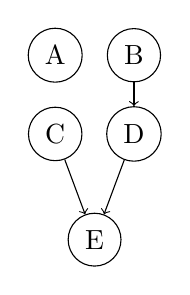
\begin{tikzpicture}[main/.style = {draw, circle}] 
		\node[main] (a) {A}; 
		\node[main] (b) [right of=a] {B};
		\node[main] (c) [below of=a] {C};
		\node[main] (d) [below of=b] {D};
		\node[main] (e) [below = of $(c)!0.5!(d)$] {E};
		\draw[->] (b) -- (d);
		\draw[->] (c) -- (e);
		\draw[->] (d) -- (e);
	\end{tikzpicture}
	\caption{Sample BN}
\end{marginfigure}
\marginnote{Consider the BN above. We will consider each variable at a time.
	\begin{itemize}
		\item[$\diamond$] $A$ has no parent, and has no descendent. Thus, \[ A \ind B, C, D, E\]
		\item[$\diamond$] $B$ has no parent, but has $D$ as a descendent. Thus, \[B \ind A, C\]
		\item[$\diamond$] $C$ has no parent, but has $E$ as a descendent. Thus, \[C \ind A, B, D\]
		\item[$\diamond$] $D$ has $B$ as a parent, and has $E$ as the descendent. Thus, \[D \ind A, C|B\]
		\item[$\diamond$] $E$ has $C$ and $D$ as parents, but has no descenent. Thus, \[I \ind A, B|C,D\]
	\end{itemize}
}
Consider the situation when each variable can take $d$ values. The naive approach gives us $\mathcal{O}(d^n)$ parameters. If we think of the potentials as probability tables (with the rows corresponding to Pa($x_i$)) and columns corresponding to the values of $x_i$, with entries as $\psi_{i}(x_i, \text{Pa}(x_i))$, we can notice that if $|\text{Pa}(x_i)| \leq k$, then the number of parameters are $\mathcal{O}(d^{k+1})$, and for $n$ variables, we have $\mathcal{O}(nd^{k+1})$, which provides us the compact representation.
\subsection{Definition}
Now we formally define these -
\begin{defn}[Bayesian Network]
A Bayesian Network is a directed graph $G = (V, E)$ together with 
\begin{itemize}[leftmargin=1cm]
	\item[$\diamond$] a random variable $x_i$ for each node $i \in V$
	\item[$\diamond$] a potential $\psi_i(x_i, \text{Pa}(x_i))$ for each node $i \in V$
\end{itemize}
\end{defn}
For a variable $x_i$ in our Bayesian Network $\mathcal G$, denote $\text{ND}(x_i)$ as the non-descendents of $x_i$. The following local conditional independencies hold in $\mathcal G$ - 
\begin{equation}
	x_i \ind \text{ND}(x_i) | \text{Pa}(x_i)
\end{equation}
Example \ref{exmp:bn-ind} shows the independencies in a simple Bayesian Network.
\begin{defn}[Factorization]	
Let $\mathcal{G}$ be a Bayesian Network graph over the variables $\{X_i\}_{i=1}^n$. We say that a distribution $P$ over the same space factorizes according to $\mathcal G$ if $P$ can be expressed as a product described in Equation \ref{eqn:factorization}. Such factorization is also known as the chain rule for Bayesian Networks, and is denoted as $\text{Factorize}(P, \mathcal G)$.
\end{defn}

\begin{defn}
Let $P$ be a distribution over $\mathcal X$. We define $\mathcal{I}(P)$ to be the set of independent assertions of the form $\mathbf X \ind \mathbf Y | \mathbf Z$ that hold in $P$.
\end{defn}
We can now write "$P$ satisfies the local independencies associated with $\mathcal  G$" as $\mathcal{I}_\ell(\mathcal G) \subseteq \mathcal{I}(P)$.
\begin{defn}[Independency-Map]
Let $\mathcal K$ be any graph object associated with a set of independencies $\mathcal{I}(\mathcal K)$. We call $\mathcal K$ an I-map for a set of independencies $\mathcal I$ if $\mathcal I(\mathcal K) \subseteq \mathcal I$.
\end{defn}
Thus for $\mathcal G$ to be an I-map for $P$, any independence that asserts in $\mathcal G$ must also assert in $P$, but $P$ can have additional independencies not reflected in $\mathcal G$.
\begin{rem}[Notation Alert]
Note that we will use the following interchangeably - $P$ satisfies the local conditional independencies satisfied by $\mathcal G$ and $\mathcal G$ is an I-map for $P$, i.e
\begin{equation}
	\text{Local-CI}(P, \mathcal G) \equiv \mathcal{I_\ell(G)} \subseteq \mathcal{I}(P)
\end{equation}
\end{rem}
\begin{thm}
Given a distribution $P(x_1, x_2, \cdots, x_n)$ and a directed acyclic graph (DAG) $\mathcal{G}$, 
\begin{equation}
\text{Local-CI}(P, \mathcal G) \Longleftrightarrow \text{Factorize}(P, \mathcal G)
\end{equation}
\end{thm}
\begin{proof}
($\implies$) We essentially need to show that if $\mathcal{G}$ is an I-map for $P$, then $P$ factorizes according to $\mathcal G$. Consider a topologically sorted order $x_1, x_2, \cdots, x_n$ in $\mathcal G$. $\text{Local-CI}(P, \mathcal G)$ tells us that $$\text{Pr}(x_i|x_{1}, \cdots, x_{i-1}) = \text{Pr}(x_i|\text{Pa}(x_i))$$
We can write
$$P(x_1, x_2, \cdots, x_n) = \prod_{i=1}^nP(x_i|x_1, \cdots, x_{i-1})$$
Each term in the product can be simplified due to the notion of Local-CI stated above, and we reach Equation \ref{eqn:factorization}, proving factorization. \\
($\impliedby$) Proof has been skipped.
\end{proof}
\subsection{Minimal Construction}
Our goal is to construct a minimal and correct BN $\mathcal G$ to represent $P$. A DAG $\mathcal G$ is correct if all Local-CIs that are implied in $\mathcal G$ hold in $P$, and a DAG $\mathcal G$ is minimal if we cannot remove any edge(s) from $\mathcal G$ and still\\ \noindent get a correct BN for $P$.
\\In the setting, we define our oracle $\mathscr{O}$ to whom we can ask any query of the type "\texttt{Is X $\ind$ Y|Z}?" pertaining to $P$ and get a boolean answer. We will query the oracle several times to build up our BN. The following algorithm constructs such a BN - \\
\begin{algorithm}[H]\label{alg:bn-con}
	\DontPrintSemicolon
	\textbf{Variables:} $x_1, x_2, \cdots, x_n \longleftarrow$ ordered variables in $\mathcal{X}$\;
	\textbf{Independencies:} $\mathcal I \longleftarrow$ set of independencies\;
	$\mathcal G \longleftarrow$ Empty graph over $\mathcal X$\;
	\For{$i=1$ to $n$}{
		$\mathbf U \longleftarrow \{x_1, \cdots, x_{i-1}\}$ \Comment{Set of candidate parents of $x_i$} \;
		\For{$U' \subseteq\{x_1, \cdots, x_{i-1}\}$}{
		\If{$U' \subset U$ and $(x_i \ind \{x_1, \cdots, x_{i-1}\} - U'|U')\in\mathcal I $}{
			$\mathbf{U} \longleftarrow U'$\;
			}	
	}
	\Comment{Now we have the minimal set $\mathbf{U}$ satisfying $(x_i \ind \{x_1, \cdots, x_{i-1}\} - \mathbf U|\mathbf U)$} \;
	\Comment{Now we set $\mathbf{U}$ to be the parents of $x_i$}\;
	\For{$x_j \in \mathbf U$}{
			Add $x_j \to x_i$ in $\mathcal G$
		}
	}
	\Return{$\mathcal{G}$}
	
	\caption{Minimal Bayesian Network Construction (I-Map)}
\end{algorithm}
We know sketch rough proofs for the claims of the algorithm.
\begin{thm}
The BN $\mathcal G$ constructed by algorithm \ref{alg:bn-con} is minimal, i.e we cannot remove any edge from the BN while maintaining the correctness of the BN for $P$.
\end{thm}
\begin{proof}
By construction. A subset of $\text{ND}(x_i)$ were available when we chose parents of $\mathbf U$ minimally.
\end{proof}
\begin{thm}
$\mathcal{G}$ constructed by the above algorithm is correct, i.e, the local-CIs induced by $\mathcal G$ hold in $P$.
\end{thm}
\begin{proof}
The construction is such that $\text{Factorize}(P, \mathcal G)$ holds everytime. Since $\text{Factorize}(P, \mathcal G) \implies \text{Local-CI}(P, \mathcal G)$, the constructed BN satisfies the local-CIs of $P$.
\end{proof}
\begin{quest}[Construction of BN]
Draw a Bayesian network over five variables $x_1,\cdots, x_5$ assuming the variable order $x_1, x_2, x_3, x_4, x_5$.
For this ordering, assume that the following set of local CIs hold in the distribution: 
\[x_1\ind x_2\quad x_3\ind x_2|x_1\quad x_4\ind x_1,x_3|x_2\quad x_5\ind x_1, x_2|x_3,x_4\]
\end{quest}
\begin{ans}
Due to the ordering, we begin by inserting $x_1$ into the BN. Then we follow Algorithm \ref{alg:bn-con} as follows:
\begin{enumerate}[leftmargin=1cm]
	\item $x_2$: Predecessor - $x_1$ \\
	\begin{itemize}[leftmargin=0.5cm]
	\item	\textit{Query 1} - Is $x_2 \ind x_1 | \emptyset$ ? :\textit{ Result 1} - True
	\end{itemize}
	Thus, $x_2$ has no parents.
	\item $x_3$: Predecessors - $x_1, x_2$
	\begin{itemize}[leftmargin=0.5cm]
		\item	\textit{Query 1} - Is $x_3 \ind \{x_1, x_2\} | \emptyset$ ? :\textit{ Result 1} - False
		\item	\textit{Query 2} - Is $x_3 \ind  x_2 | x_1$ ? :\textit{ Result 2} - True
	\end{itemize}
	Thus, $x_3$ has $x_1$ as a parent, and $x_2$ as a non-descendent.
	\item $x_4$: Predecessors - $x_1, x_2, x_3$
	\begin{itemize}[leftmargin=0.5cm]
		\item	\textit{Query 1} - Is $x_4 \ind \{x_1, x_2, x_3\} | \emptyset$ ? :\textit{ Result 1} - False
		\item	\textit{Query 2} - Is $x_4 \ind  \{x_2, x_3\} | x_1$ ? :\textit{ Result 2} - False
		\item	\textit{Query 3} - Is $x_4 \ind  \{x_1, x_3\} | x_2$ ? :\textit{ Result 3} - True
	\end{itemize}
	Thus, $x_4$ has $x_2$ as a parent, and $x_1, x_3$ as non-descendents.
	\begin{marginfigure}\label{fig:bn-example}
		\centering
		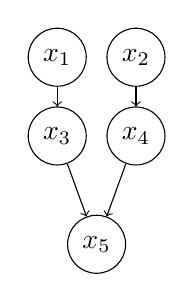
\begin{tikzpicture}[main/.style = {draw, circle}] 
			\node[main] (a) {$x_1$}; 
			\node[main] (b) [right of=a] {$x_2$};
			\node[main] (c) [below of=a] {$x_3$};
			\node[main] (d) [below of=b] {$x_4$};
			\node[main] (e) [below = of $(c)!0.5!(d)$] {$x_5$};
			\draw[->] (a) -- (c);
			\draw[->] (b) -- (d);
			\draw[->] (c) -- (e);
			\draw[->] (d) -- (e);
		\end{tikzpicture}
		\caption{BN Example}
	\end{marginfigure}
	\item $x_5$: Predecessors - $x_1, x_2, x_3, x_4$ \\
	Check that it has $x_3, x_4$ as parents and $x_1, x_2$ as non-descendents.
\end{enumerate}
Thus, finally we get the BN as in Figure \ref{fig:bn-example}
\end{ans}


\begin{rem}[Importance of ordering]
It is possible that a different ordering in $\mathcal X$ gives rise to a different BN, which although may be minimal, but may not be \textit{optimal}. A minimal BN is defined for a given ordering, while an optimal BN is defined over all orderings. Example \ref{exmp:bn-order} shows such a case.
\end{rem}
\begin{exmp}\label{exmp:bn-order}
To be added
\end{exmp}
\subsection{D-Separation}
Our goal is to know when we can guarantee $\mathbf X \ind \mathbf Y|\mathbf Z$ holds given a BN  $\mathcal G$. The further discussion provides some cases where we can guarantee $\mathbf X\; \cancel\ind\; \mathbf Y|\mathbf Z$.
\begin{marginfigure}
\begin{center}
	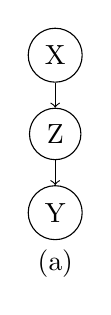
\begin{tikzpicture}[main/.style = {draw, circle}] 
	\node[main] (x) {X};
	\node[main] (z)[below of=x] {Z};
	\node[main] (y)[below of=z, label=below:(a)] {Y};
	\draw[->] (x) -- (z);
	\draw[->] (z) -- (y);
	\end{tikzpicture}
	\hspace{1cm}
	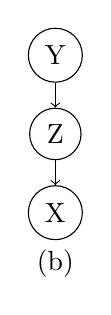
\begin{tikzpicture}[main/.style = {draw, circle}] 
		\node[main] (y) {Y};
		\node[main] (z)[below of=y] {Z};
		\node[main] (x)[below of=z, label=below:(b)] {X};
		\draw[->] (y) -- (z);
		\draw[->] (z) -- (x);
	\end{tikzpicture}
\end{center}
\caption{Causal and evidential effect}
\end{marginfigure}
\begin{marginfigure}
	\begin{center}
		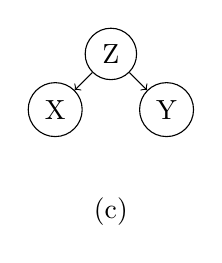
\begin{tikzpicture}[main/.style = {draw, circle}] 
			\node[main] (z) {Z};
			\node[main] (x)[below left of=z] {X};
			\node[main] (y)[below right of=z] {Y};
			\draw[->] (z) -- (x);
			\draw[->] (z) -- (y);
			\node (e) [below = of $(x)!0.5!(y)$] {(c)};
		\end{tikzpicture}
		\hspace{0.5cm}
		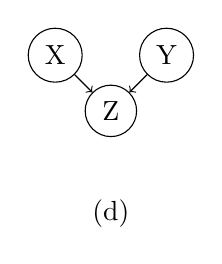
\begin{tikzpicture}[main/.style = {draw, circle}] 
			\node[main] (z) {Z};
			\node[main] (x) [above left of=z] {X};
			\node[main] (y)[above right of=z] {Y};
			\draw[->] (y) -- (z);
			\draw[->] (x) -- (z);
			\node (e) [below = of $(z)$] {(d)};
		\end{tikzpicture}
	\end{center}
	\caption{Common cause and common effect}
\end{marginfigure}
\begin{enumerate}
	\item \textbf{Direct Connection:} If there is an edge $X \to Y$, then regardless of any $\mathbf Z$, we can find examples where they influence each other.
	\item \textbf{Indirect Connection:} This means that there is a trail between the nodes in the graph. We consider the simple case when we a 3-node graph and $Z$ is between $X$ and $Y$. Consider the 4 diagrams to the left for reference.
	\begin{enumerate}
		\item \textit{Indirect causal effect:} $X$ cannot influence $Y$ via $Z$ if $Z$ is observed.
		\item \textit{Indirect evidential effect:} This is similar to the previous case as dependence is a symmetric notion. Thus, $X$ can influence $Y$ via $Z$, only if $Z$ is not observed.
		\item \textit{Common cause:} The conclusion is similar to (a) and (b).
		\item \textit{Common effect:} (v-structure) This case is a bit tricky to understand, but the crux is that $X$ can influence $Y$ when either $Z$ or one of $Z$'s descendents is observed.
	\end{enumerate}
If we have flow of influence from $X$ to $Y$ via $Z$, we say that the trail $X \rightleftharpoons Y \rightleftharpoons Z$ is active.
	\begin{equation}\label{eqn:dsep}
	\begin{split}
	&\begin{rcases}
		\text{Causal trail: }& X \to Z \to Y\\
		\text{Evidential trail: }&Y \to Z \to X \\
		\text{Common cause: }& X \leftarrow Z \to Y \\
	\end{rcases} \text{Active if and only if $Z$ is observed}\\
&\begin{rcases}
	\star \;\;	\text{Common effect: } X \to Z \leftarrow Y
\end{rcases} \\
&\hookrightarrow \text{Active if and only if $Z$ or one of $Z$'s descendent is observed}
	\end{split}
	\end{equation}
\end{enumerate}
Now, we can create a general notion of trails -
\begin{defn}
Let $\mathcal G$ be a BN, and $x_1 \rightleftharpoons \cdots \rightleftharpoons x_n$ be a trail in $\mathcal G$. Let $\mathbf Z \subset \{\text{observed variables}\}$. The trail is active given $\mathbf Z$ if
\begin{itemize}[leftmargin=1cm]
	\item[$\diamond$] Whenever we have a v-structure $x_{i-1} \to x_i \leftarrow x_{i+1}$, then $x_i$ or one of its descendents are in $\mathbf Z$
	\item[$\diamond$] No other node along the trail is in $\mathbf Z$.
\end{itemize}
We can see that if $x_1 \in \mathbf Z$ or $x_n \in \mathbf Z$, then the trail is inactive.
\end{defn}
\marginnote{Essentially in a DAG, $\mathbf Z$ d-separates $\mathbf X$ from $\mathbf Y$ if all paths $\mathcal P$ from any $\mathbf X$ to $\mathbf Y$ is blocked by $\mathbf Z$.\\A path $\mathfrak{P}$ is \textit{blocked} if it is inactive, i.e there is no flow of influence.}
\begin{defn}[d-separation]
Let $\mathbf X, \mathbf Y, \mathbf Z$ be three sets of nodes in $\mathcal G$. We say that $\mathbf X$ and $\mathbf Y$ are d-separated given $\mathbf Z$, i.e $\text{d-sep}_\mathcal{G}(\mathbf X; \mathbf Y|\mathbf Z)$ if there is no active trail between any node $x \in \mathbf X$ and $y \in \mathbf Y$ given $\mathbf Z$.
\end{defn}
\marginnote{We use the same notation as $\mathcal{I}(P)$ as we can show that the independencies in $\mathcal{I}(\mathcal G)$ are those guaranteed to hold for every distribution over $\mathcal G$ (Theorem \ref{thm:global-markov-ind}).}
\begin{defn}[Global Markov independencies]
The set 
\begin{equation}
\mathcal{I(G)} \overset{\mathrm{def}}{=} \{(\mathbf X \ind \mathbf Y | \mathbf Z): \text{d-sep}_\mathcal{G}(\mathbf X; \mathbf Y | \mathbf Z)\}
\end{equation}
denoting the set of independencies corresponding to d-separation is the set of global Markov independencies. 
\end{defn}
\begin{thm}\label{thm:global-markov-ind}
The d-separation test identifies the complete set of conditional independencies that hold in all distributions that conform to a given Bayesian Network.
\end{thm}
\begin{proof}
Skipped.
\end{proof}
Now, we look at another way to check d-separation over BNs, but first we define some terms.
\begin{defn}[Ancestral Graph]
Given a graph $G = (V,E)$ and a set of nodes to focus on, say $V^* \subseteq V$, the ancestral graph ${G}^A$ is a subgraph induced by $V^A = V^* \cup \mathcal{A}(V^*)$ where $\mathcal{A}(V^*)$ denotes the ancestors of $V^*$. Thus,
\begin{equation}
G^A = G\braket{V^A} = (V^A, \{(u,v) | (u, v) \in E \text{ and } u, v \in V^A\})
\end{equation}
\begin{defn}[Markov Blanket]
Given a random variable $Y$ in a random variable set $\mathcal X = {X_1, X_2, \cdots, X_n}$ , it's Markov Blanket is any subset $\mathcal S$ of $\mathcal X$, conditioned on which other variables are independent with $Y$, i.e
\begin{equation}
Y \ind \mathcal{X}\setminus\mathcal{S} | \mathcal S
\end{equation}
Thus, we can infer $Y$ from $\mathcal S$ itself, and the rest of the elements are redundant in observation.
\end{defn}
\marginnote{\begin{rem}\label{rem:bn-moral}Essentially we are finding an equivalent undirected graph for a DAG. We find all pairs of non-adjacent nodes having a common child, and add an undirected edge between them. Then we transform all directed edges in the resulting graph to undirected edges. \end{rem}}
\end{defn}
\begin{defn}[Moral graph]
A moral graph of a directed acyclic graph $G$ is an undirected graph in which each node of the original $G$ is now connected to its \textit{Markov Blanket}.
\end{defn}
\begin{algorithm}[H]\label{alg:bn-moral}
	\DontPrintSemicolon
	\textbf{Given:} Bayesian Network $\mathcal G$, Condition to check $\mathcal{C}$: $\mathbf X \ind \mathbf Y | \mathbf Z$ \;
	$\mathcal C \leftarrow$ False\;
	$G = (V,E) \leftarrow$ Underlying DAG in $\mathcal G$. \;
	$G^A = (V^A, E^A) \leftarrow$ Ancestral graph of $G$ \;
	$G^A_M = (V^A_M, E^A_M)\leftarrow$ Moral graph of $G^A$ using Note \ref{rem:bn-moral} \;
	\Comment{Delete the nodes in $\mathbf Z$ and all its connections}\;
	\For{$z \in \mathbf Z$}{
		$\Xi \leftarrow \{\}$\;
		\For{$u \in V$ such that $\xi=(u, z) \in E^A_M$}{
			$\Xi \leftarrow \Xi \cup \xi$\;
		}
		$E^A_M \leftarrow E^A_M \setminus \Xi$\;
		$V^A_M \leftarrow V^A_M \setminus \{z\}$\;
	}
	\If{$\mathbf X$ and $\mathbf Y$ are disconnected in the resulting graph}{
		$\mathcal C \leftarrow$ True\;
	}
	\caption{Checking for independence in a BN}
\end{algorithm}

	% rem defn proof prop exmps quest
\end{document}
